\chapter{L'environnement du stage, la Société pour l'Informatique Industrielle}

\section {Introduction}
Ce chapitre vise à apporter au lecteur une compréhension suffisante du contexte du stage pour en saisir les enjeux. 

Il s'attache d'abord à décrire la structure d'accueil, à savoir le groupe \gls{SII}, au sein duquel s'articulent les agences françaises et en particulier, l'agence \^{I}le-de-France.
Cette dernière englobe la structure berruyère qui a hébergé le stage. \`{A} ce titre, sa portée et son organisation seront particulièrement détaillées. 

Nous spécifierons ensuite les axes stratégiques qui justifient la mise en oeuvre du projet. 
Une section décrira l'apport souhaité du projet pour SII tandis que la section suivante reviendra sur un acteur particulier de l'écosystème de l'entreprise : l'INSA Centre Val-de-Loire, qui s'inscrit en partenaire financier, 
stratégique et organisationnel en amont de ce projet.

\section{Principaux repères et évolution de la structure SII}

\subsection{Signalétique générale : du groupe à l'agence parisienne}

Couramment nommée \gls{SII}, la Société pour l'Informatique Industrielle est une \gls{SA}, aujourd'hui implantée dans dix-huit pays, sur quatre continents.

Sur l'exercice 2015/2016, le groupe SII enregistre un chiffre d'affaires consolidé de 360,1M\euro\cite{Bib_exercice_2015_2016}, pour un résultat net de 13.13M\euro\cite{Bib_exercice_2015_2016}, et compte sur un effectif moyen de 5 226 collaborateurs\cite{Bib_exercice_2015_2016}. 

Depuis plus de 30 ans\cite{Bib_exercice_2015_2016}\cite{Bib_memento_ag_idf}, SII \oe{}uvre pour s'inscrire en tant que partenaire technologique de choix auprès d'une clientèle professionnelle diversifiée. 
Le groupe --qui a consolidé son expérience dans quatorze secteurs d'activités disctincts-- propose des offres liées aux savoir-faire suivants : 

\begin{itemize}
 \item \textbf{L'informatique embarquée} incluant le développement de logiciels embarqués, de contrôle commande ou encore de bancs de tests   
 \item \textbf{L'ingénierie scientifique} qui balaye les champs de l'électronique, du traitement du signal et de la mécanique
 \item \textbf{Les \gls{NTIC}}, englobant les problématiques de téléphonie, de web, de mobilité ou d'infrastructures diverses
 \item \textbf{Les Systèmes d'Informations} qui recouvrent l'informatique décisionnelle, financière ou la sécurité du \gls{SI}
\end{itemize}

Les secteurs d'activités s'organisent quant à eux en \gls{BU}. Chacune de ces unités s'adresse à un groupe de clients majeurs et détient un organigramme interne, placé sous la responsabilité du Directeur de \gls{BU}. 

L'agence Île-de-France est une des neuf agences françaises de la société. Elle est placée sous la responsabilité du Directeur d'Agence, M. Didier Bonnet.
Son administration est abritée sur le site de Kennedy\footnote{104 Avenue du Président Kennedy, 75016 Paris} --principalement dédié aux opérations de gestions-- et recouvre deux sites supplémentaires : celui du 
Dynasteur\footnote{6, 12, 10 Rue Andras Beck, 92360 Meudon} et celui de Bourges\footnote{14, allée Charles Pathé, 18000 Bourges } au sein duquel s'est déroulé ce stage. 

Les activités de réalisations se concentrent pour cette agence autour de quatre secteurs d'activités qui sont présentés figure \ref{fig:BU-IDF}. 

\begin{figure}[h]
  \centering
    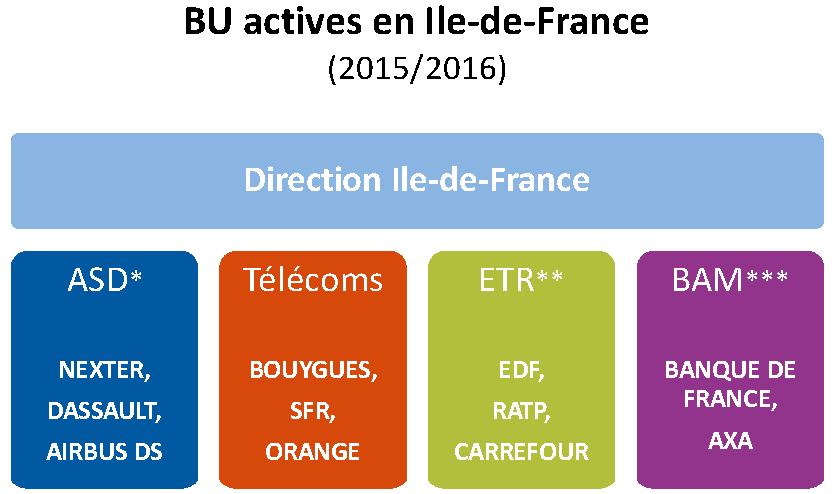
\includegraphics[width=.5\linewidth]{figures/BU-clients-IDF}
    \caption*{*Aero-Space Defense, **Energie Transport Retail, ***Banque Assurance Mutuelle}  
  \captionof{figure}{BU actives en IDF}
  \label{fig:BU-IDF}
\end{figure}

Pour ces secteurs, un portefeuille de dix clients est responsable de 80\% du chiffre d'affaires annuel de l'agence. 
La figure \ref{fig:BU-IDF} donne la nomenclature des \gls{BU} définies par l'entreprise, et illustre la clientèle française qui leur est associée.  

\subsection{\'{E}volution de SII en France et à Bourges}

SII a été créée à Paris en 1979 par un ingénieur, Bernard Huvé, qui en est aujourd'hui le Président du Conseil de Surveillance. 
S'en suivra la création de multiples agences provinciales, jusqu'en 1999 où, forte de 400 collaborateurs et d'une croissance soutenue, la société s'introduit en bourse.  
On peut relever l'internationalisation de SII, qui intervient en 2006 avec l'ouverture d'une filiale en Pologne, pour atteindre aujourd'hui un total de 17 filiales à l'étranger\cite{Bib_exercice_2015_2016}.  

Dans ce qui va suivre, nous nous concentrons uniquement sur l'implantation française de SII, qui se retrouve à présent au travers 22 sites sur le territoire.  

\begin{figure}[h]
    \centering
    
\includegraphics[width=.5\linewidth]{figures/BU-IDF}
    \captionof{figure}{Répartition sectorielle de SII en IDF\cite{Bib_memento_ag_idf}}
    \label{fig:Rep-sectorielle}
\end{figure}

Aujourd'hui, les secteurs d'activités clés de l'entreprise peuvent être classés selon deux catégories\cite{Bib_memento_ag_idf}, que la figure \ref{fig:Rep-sectorielle} permet de justifier : 

\begin{itemize}
  \item \textbf{Les secteurs stratégiques}, que sont \gls{ASD} et Télécoms. Etant des générateurs forts de valeur, ils concernent des marchés mûrs où SII a su établir des relations pérennes avec ses clients grand-compte. 
  \item \textbf{Les secteurs de conquête}, inclus dans les \gls{BU} \gls{ETR} et \gls{BAM}, amenés à se digitaliser massivement
\end{itemize}

Dirigée par M. Fabrice Bosch, l'agence berruyère compte quant à elle une cinquantaine de collaborateurs répartis sur les secteurs d'activités \gls{ETR} et \gls{ASD}. 
Elle héberge également des activités de \gls{QHSE} sous la responsabilité de M. Jean-Sébastien Salis.  

Les activités \gls{ETR} se concentrent sur le développement de solutions billetiques pour des acteurs majeurs du transport de voyageurs. 
En parallèle, les activités \gls{ASD} sont tournées vers un ensemble d'acteurs du secteur de l'armement et de la Défense historiquement implantés à Bourges et, aujourd'hui encore, essentiels à l'économie locale\cite{Bib_def_cher}. 
Parmi ces clients ont peut citer la filiale missilière du groupe Airbus MBDA, ou encore Nexter Munitions dont le site de Bourges accueille les ingénieurs et cadres affilés aux missions de \gls{RD} . 
Enfin, et au regard du caractère critique des missions relevant de la défense nationale ou européenne, on notera que le site de Bourges dispose d'une habilitation à mener au sein de son infrastructure des projets classés Confidentiel
Defense. 

\section{Une mission R\&D pour b\^{a}tir de nouvelles offres}

\subsection{SII Research dans l'agence berruyère}

La mission qui m'a été confiée durant ce stage est placée sous l'égide de l'entité SII Research. 
Sous la responsabilité du Pôle Innovation, cette structure permet de mener à bien des projets transverses aux différents secteurs d'activités, financés sur les fonds propres de l'entreprise.  

Typiquement, ce type de projet sera qualifié de \gls{POC} ou démonstrateur. Pour l'entreprise d'accueil, les réalisations sont menées avec les objectifs suivants : 

\begin{itemize}
  \item Valoriser l'expertise de l'entreprise dans des domaines techniques précis et actuels
  \item Elargir les connaissances internes en communiquant autour des savoir-faire sollicités
  \item Bâtir de nouvelles offres à partir de tout ou partie du \gls{POC} 
\end{itemize}

Ces réalisations permettent de communiquer techniquement avec des acteurs internes et des parties prenantes externes (clients, prospects ou étudiants) --notamment par le biais de médias sociaux-- sans compromettre la confidentialité 
de projets clients. 

Ce projet s’inscrit dans la mise en \oe{}uvre d’un Système Robotique Tactique Multi Missions pour le Surveillance et l’Aide à la Prise de Décisions dans les Milieux à Risques, adressé au secteur de la Défense 
et, plus particulièrement, aux clients berruyers de la \gls{BU} \gls{ASD}.
Dans cette optique, le stage s'est d'emblée accompagné de l'objectif ambitieux d'être véhiculé auprès de représentants de l'entreprise Nexter Systems, à son terme ou durant des stages suivants.  
Ainsi, plusieurs jalons ont pu être posés avec succès dans le respect des procédures internes de validations hiérarchiques. 
Il a notamment pu être présenté à MM. Giraud-Sauveur et Boucher respectivement commercial / chargé d'affaires sur le périmètre MBDA / Nexter et Directeur de projets Nexter. 
Accompagné d'une démonstration, cet entretient s'est soldé positivement et a permis au \gls{POC} d'être relayé par la suite aurpès des instances susceptibles d'assurer son pilotage futur.  

\subsection{Fruits du partenariat avec l'INSA Centre Val-de-Loire}

Ce stage --comme celui d'Alban Chazot-- s'effectue dans le cadre d'un partenariat entre SII et l'INSA Centre Val-de-Loire. 
La relation établie entre ces deux entités découle de la convention ``Carré des partenaires'' acceptée par les deux parties en 2015.
Quentin Ménart, aujourd'hui ingénieur logiciel au sein de l'agence SII Bourges nous a précédés en expérimentant l'année dernière un stage découlant du partenariat.  

Cette relation privilégiée mène à retrouver SII en qualité d'acteur ou de sponsor de certains évènements majeurs de la vie étudiante : Nuit de l'Info, Forum des entreprises, conférences techniques.
Par ailleurs, elle permet de favoriser l'accueil de stagiaires et d'alternants en provenance de l'institut.  

\begin{figure}[h]
    \centering
    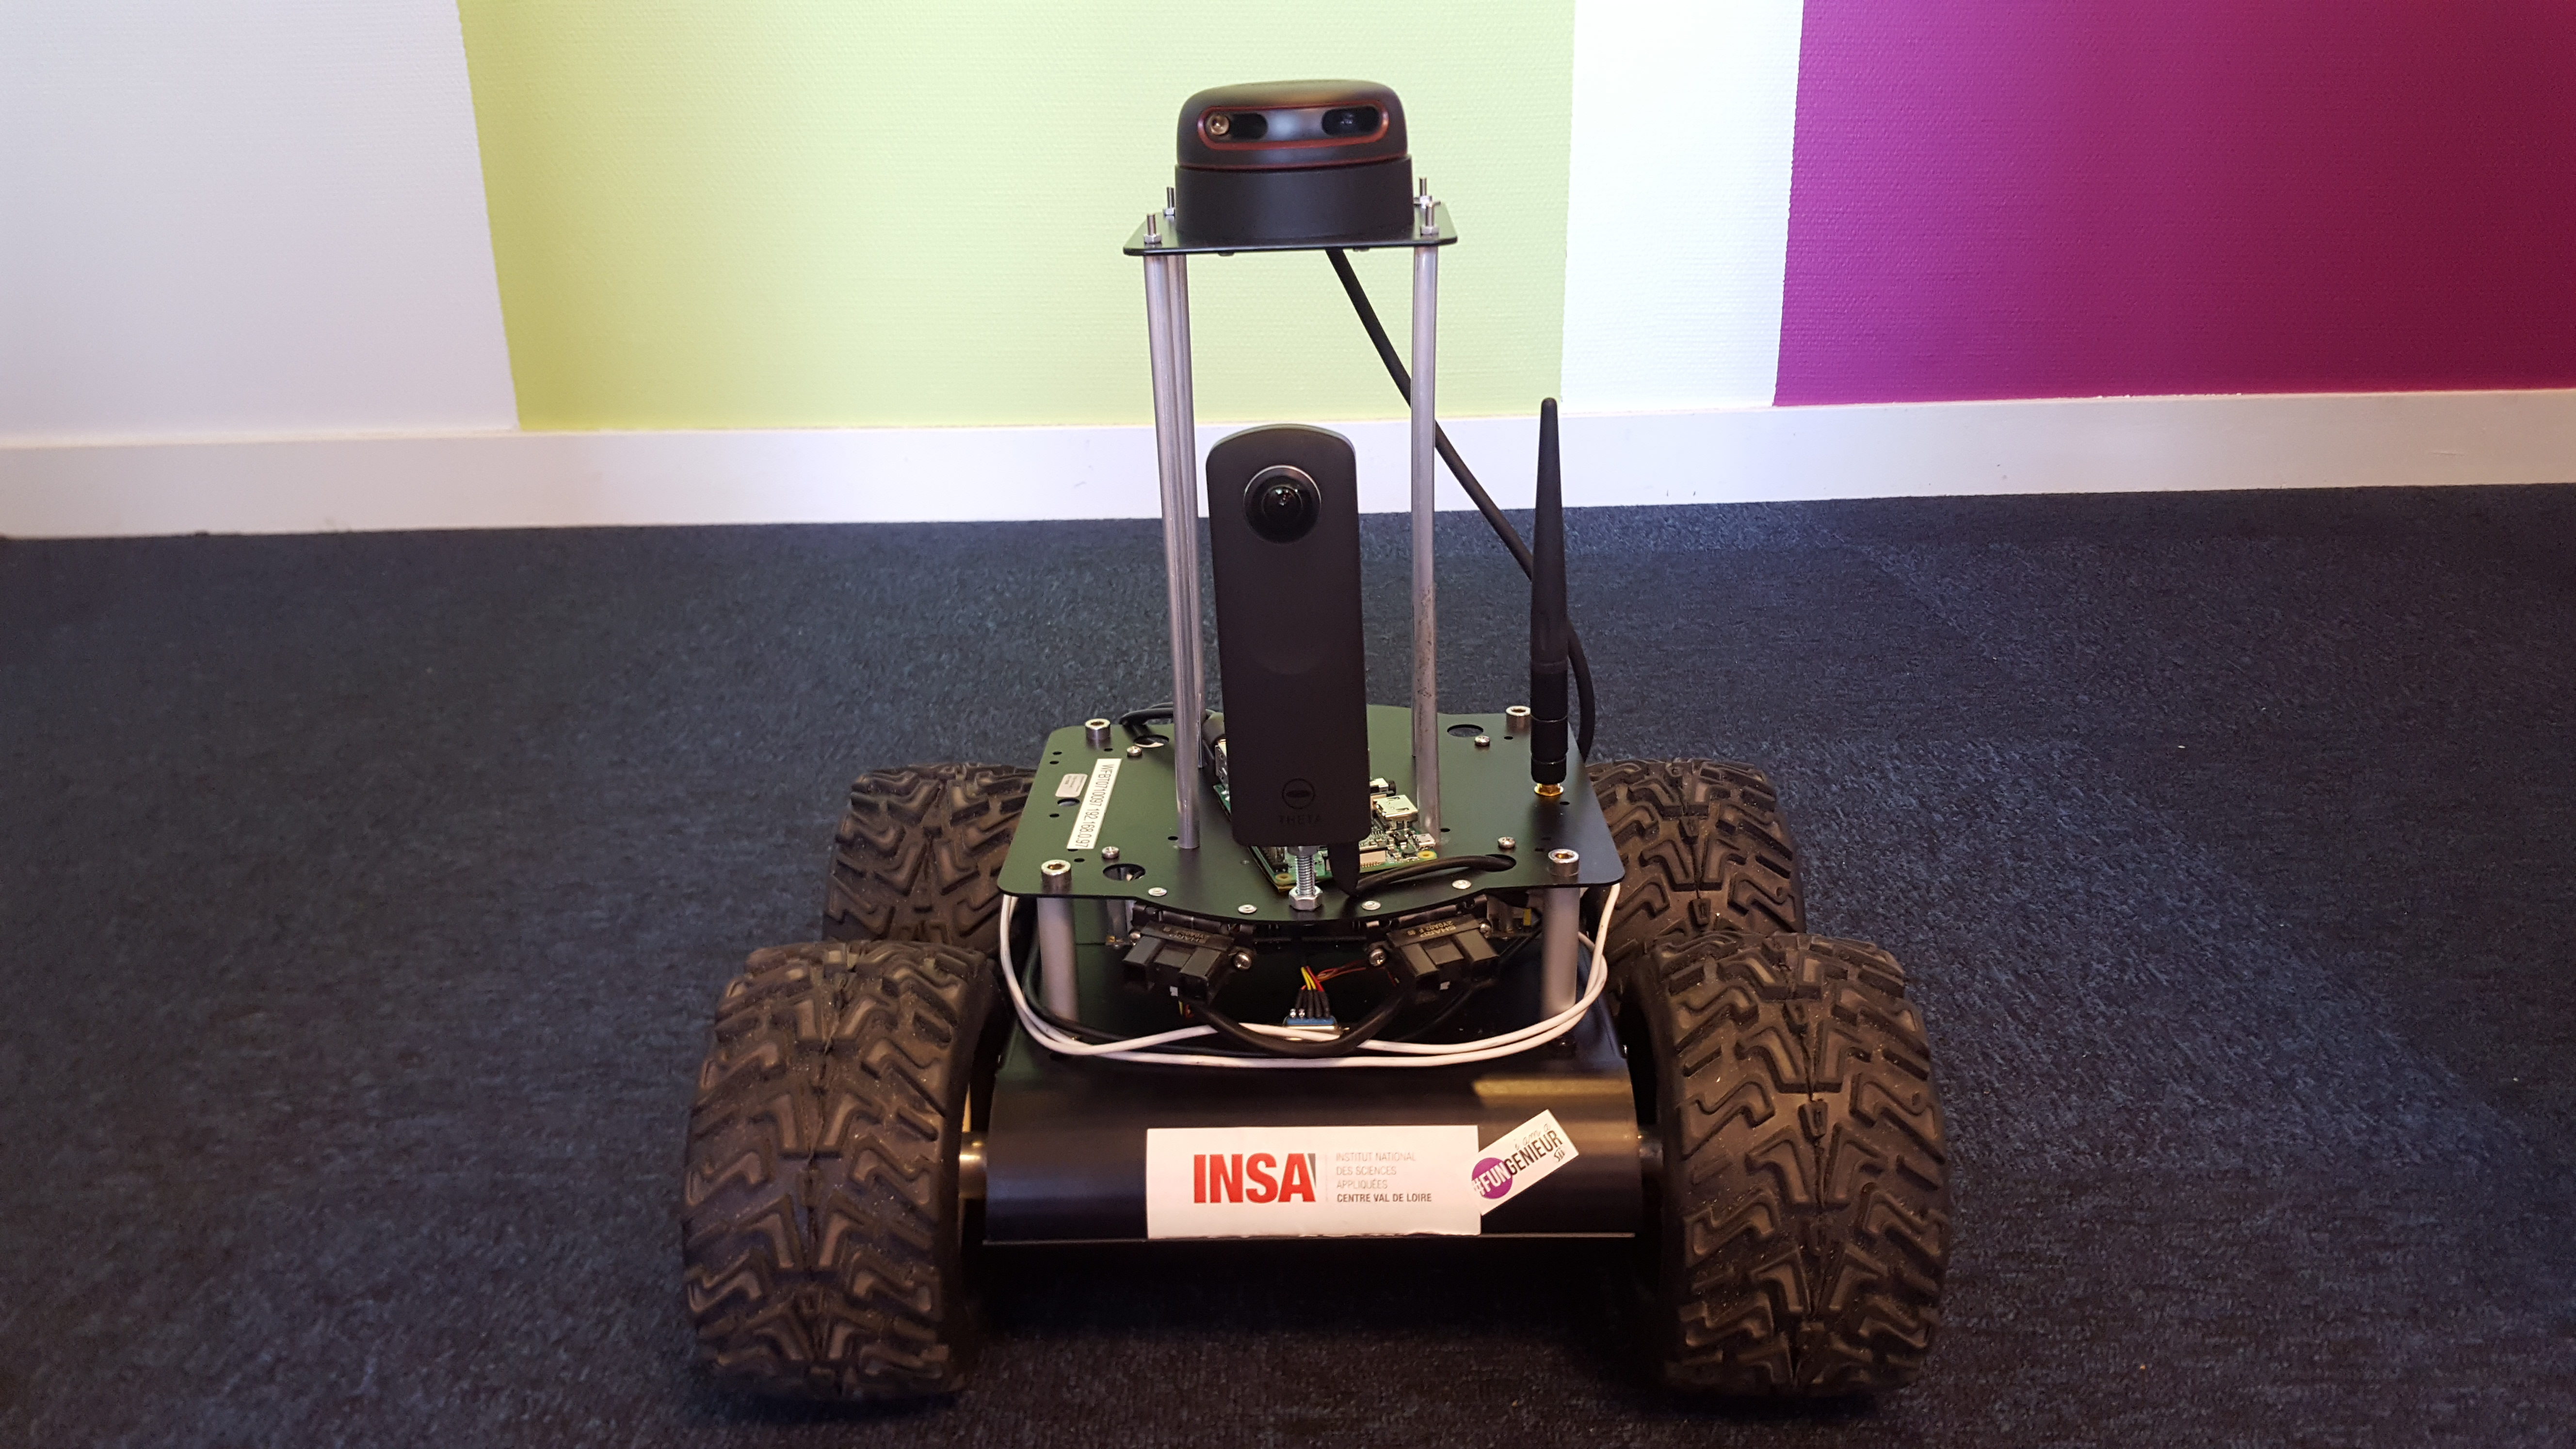
\includegraphics[width=.4\linewidth]{figures/wifibot}
    \captionof{figure}{Wifibot embarquant un RPLidarA2 et une caméra Theta S}
    \label{fig:Wifibot}
\end{figure}

En ce qui nous concerne, cette collaboration a impacté nos stages de manière visible et fructueuse.
En effet, elle a permis le prêt d'un robot mobile par M. Benali Abderraouf, enseignant-chercheur en robotique à l'INSA Centre Val-de-Loire. 
Ce robot qui a constitué la base du projet est présenté sur la figure \ref{fig:Wifibot}.
Dans ce cadre, l'INSA Centre Val-de-Loire a également financé pour moitié le matériel nécessaire au projet, à savoir une caméra Theta S à 360\degre (cf. figure \ref{fig:Wifibot}).

Ce partenariat a aussi donné lieu à des réunions régulières de co-pilotage de projet réunissant MM. Hafiane et Bosch. 
Elles nous ont permis de réfléchir ensemble au cap à donner, au matériel à acquérir ou encore aux techniques à employer.
Enfin, nous avons pu évoluer sereinement en qualité de stagiaires, en comptant sur le suivi fréquent de M. Adel Hafiane, tant dans la mise en place du projet, que durant les phases plus tardives de développement.
